\documentclass[12pt]{article}
\usepackage{a4wide}
\usepackage{graphicx}
\usepackage{mathtools}
\usepackage{placeins}
\usepackage{parskip}
%\usepackage{fullpage}
\usepackage{epstopdf}
\usepackage[margin = 1.0in]{geometry}
\usepackage[font=small,labelfont=bf]{caption}

\usepackage[toc]{appendix}

\usepackage{listings,xcolor}
\usepackage[nottoc]{tocbibind}

\lstset{language=Java}
\lstset{basicstyle={\sffamily\footnotesize},
  numbers=left,
  numberstyle=\tiny\color{gray},
  numbersep=5pt,
  breaklines=true,
  captionpos={t},
  frame={lines},
  rulecolor=\color{black},
  framerule=0.5pt,
  columns=flexible,
  tabsize=2
}

\begin{document}

\pagenumbering{gobble}

\begin{minipage}[b]{110mm}
        {\Huge\bf School of Physics\\ and Astronomy
        \vspace*{17mm}}
\end{minipage}
\hfill
\begin{minipage}[t]{40mm}               
        \makebox[40mm]{
        
\includegraphics[width=40mm]{crest.eps}}
\end{minipage}

\vspace*{2cm}
\begin{center}
        \Large\bf \Large\bf MPhys Project\\
        \LARGE\bf Statistical Physics of Replication Dynamics
\end{center}
\vspace*{0.5cm}
\begin{center}
        Alistair Jones\\  
        {\bf Supervisor:} Dr. R. A. Blythe \\          
        March 2015     
\end{center}

\begin{center}
\subsection*{Abstract}
\end{center}

\newpage
\tableofcontents

\newpage
\pagenumbering{arabic}

\section{Introduction}


\newpage
\section{Background, motivation and aims}
This investigation was concerned with the behaviour of language in speech communities. When members of a community, or \emph{speakers}, interact there are numerous possible linguistic objects and structures, e.g. words, phrases or idioms, which can be used to express particular meanings. In many cases an individual may have to choose one linguistic object out of a number of alternatives with the same meaning. For example, `couch', `sofa' and `chesterfield' are all words that refer to the same physical object. The focus of this study was on exploring how such choices are made and, more specifically, how preferences towards a particular way of expressing certain meanings emerge based on interactions between individuals. 

\subsection{Selection mechanisms}
Language change can be modelled as a two-step evolutionary operation, consisting of the generation of variations and the propagation of such variations through the speech community \cite{croft}. The variations produced are known as \emph{variants} of a particular \emph{linguistic variable}. Variants corresponds to the linguistic objects and structures mentioned previously, while the variable corresponds to the associated meaning. In the above example, the words `couch', `sofa' and `chesterfield' are the variants and the physical object they correspond to is the linguistic variable. The fundamental dynamical process of this evolutionary procedure is replication, in particular the replication of linguistic objects and structures, or variants, through speech. Speaking a collection of variants is referred to in the following as producing an \emph{utterance}. Each time a speaker produces an utterance he/she replicates variants they have heard before. In other words, this replication process is controlled by the speaker and their knowledge of the language, which has been previously determined by the language he/she has been exposed to. The interactions a particular speaker has experienced in the past will therefore influence those in the future, i.e.\ a speaker builds a usage-based memory of the variants which controls the outcome of future interactions. 

The central element in processes of the type above is unit of replication, called the \emph{replicator} \cite{hull}. An example of a replicator in biological evolution would be a gene, which is replicated during the production of sex cells (meiosis) and passed on to the offspring of an individual. In language change the replicator is a variant, which is replicated during speech interactions between individuals \cite{lc&v}.\ \emph{Selection} is the process which determines the frequencies with which different replicators are replicated. In general it can be argued that \emph{interactors} are also required for selection to occur \cite{hull}. Returning to the example of biological evolution, the interactors are organisms which are responsible for replication through interactions between one another. In other words, an organism reproducing means that it's genes are replicated and are thus propagated throughout a population, otherwise the genes will become extinct. Similarly, in language change the speakers are the interactors which replicate certain variants; if speakers select to replicate one variant more than another then the unused variant will eventually become extinct. Note the subtle difference between these two system types: in biology a replicator (a gene) "belongs to" an interactor (an organism), where the survivability of a replicator is due to the "fitness" of the interactor; in linguistic theory however, there is no one-to-one relationship between a replicator (a variant) and the speaker who produces it and the replicator's survivability arises from the social standing (i.e.\ the influence different speakers have over others in the community) of the individuals using that variant.

The theory of utterance selection, as presenting in \cite{croft}, distinguishes between two forms of selection: \emph{interactor selection} and \emph{replicator selection}. Interactor selection labels the fact that an interactor may be influenced by some interactors more than others. The difference in influence can be due to either the frequency with which certain interactors interact, i.e.\ the more often two individuals interact the greater their influence on one another, or the interaction of an interactor with a particularly strongly influential individual. The former can be thought of, in context of language behaviour, as an individual interacting with their neighbour more than with someone from another town, while an example of the latter would be the influence over an individual a friend has in contrast to an acquaintance. Replicator selection stems from the replicator and corresponds to the preference of an interactor towards a particular replicator. Replicator selection is thus an intrinsic property of a replicator. In a speech community, an example may be when a speaker prefers to use words or phrases commonly used by speakers they wish to associate with. 

In summary: variants of linguistic variables and speakers correspond to replicators and interactors respectively with interactions propagating replicators through the community; during speech a speaker utters a collection of variants which are replicated; variants are selected according a speaker's usage-based knowledge of the language, which arises as a consequence of the two sources of selection discussed above; the action of selection during each interaction alters a speakers knowledge of the language and thus influences the frequencies with which certain variants will be replicated in future; consequently it is possible for a variant to out-compete others, i.e. for the community to collectively reach a consensus as to which variant they use.

\subsection{History of language change}
While the above discussion may seem somewhat abstract, the underlying motivation for studies of this type is entirely physical. To illustrate this point, recall the above example regarding the variety of alternatives to object one might call a `sofa'. Figure \ref{sofa} shows data from a study into the usage of the words `sofa', `chesterfield', `couch', `davenport' and `setee' in Canadian English. This was an apparent-time study which means data was collected from speakers of different ages, with older speakers taken to be representative of the typical behaviours at appropriate points in the past. Plotting the data in reverse age order thus gives an estimate of the actual change in usage frequency over time, as the 90 year old speakers represent roughly 90 years in the past and so on.

\begin{figure}[h]
\begin{center}
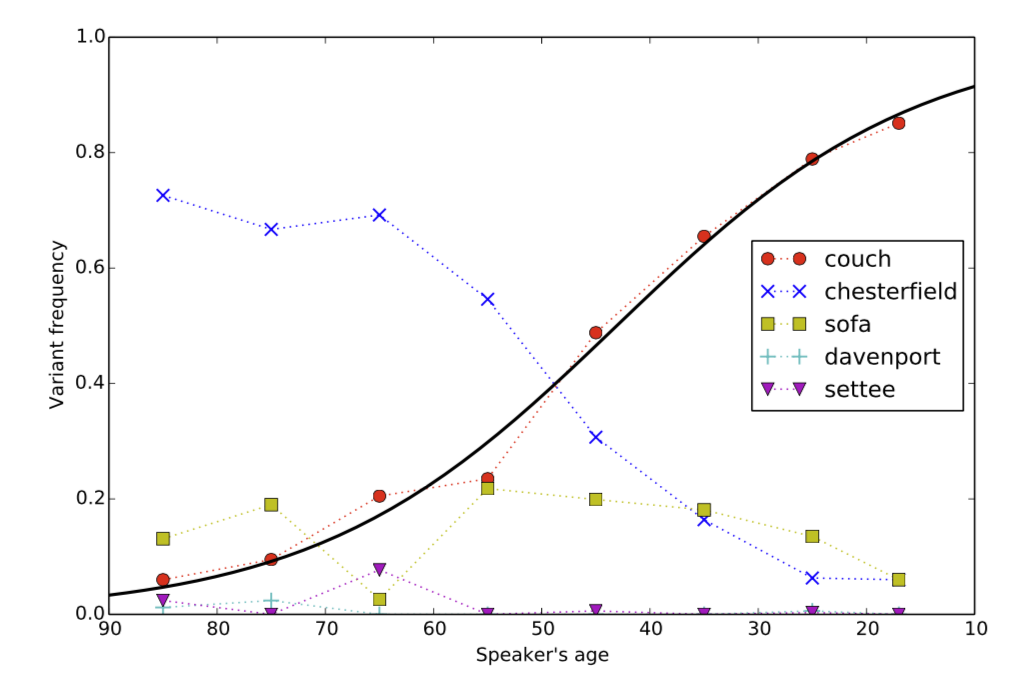
\includegraphics[width=\textwidth]{sofa.png}
\end{center}
\caption{Variation in usage frequency of different furniture terms in Canadian English. Data collected using an apparent-time study, meaning data collected from speakers of different ages with older speakers taken to be representative of typical behaviour at an appropriate time in the past. Plotting the data in reverse age order thus gives an estimate of the actual change in usage frequency over time. Data originally from \cite{20}.}\label{sofa}
\end{figure}

The key feature to observe is the shape of the curves for the usage frequency of the two variants `couch' and `chesterfield'. Notice that the usage frequency of `chesterfield' is much greater among 90 year old speakers ($>70\%$) than 10 year old speakers ($<10\% $) while the converse true for `couch', where the minority of 90 year old speakers ($<10\% $) and the vast majority of 10 year old speakers ($\approx 90\%$) are users. In other words, over time the community's preferences changes from `chesterfield', referred to as the \emph{outgoing variant}, to `couch', referred to as the \emph{incoming variant}. The usage frequencies are said to follow an `S-curve trajectory' \cite{Scurve}: the rate of growth initially accelerates until both the incoming and  the outgoing variant are widely used, after which the rate of growth decelerates as the incoming variant becomes used by the majority of speakers. 

This example motivates the inclusion of replicator selection in the theory of utterance selection discussed previously. Recall that interactor selection is due to individuals being influenced by the utterances of some speakers more than others and replicator selection is selection due to an intrinsic preference of a speaker towards a particular variant. While interactor selection is quite physically intuitive, e.g.\ one can picture a scenario in which a person will interact with some people more than others, it is not clear that replicator selection corresponds to anything physical. However, previous studies have found that, in order to reproduce the S-curve trajectories above, both interactor and replicator selection are required \cite{ref2}. There exist other empirical features of language change for which this is also true, such as the rapid rate of change of new-dialect formation \cite{ref1} or that the time-scales over which conventions remain stable are highly diverse \cite{ref3}, although these are not discussed here. Reproducing these behaviours relies more specifically on the community reaching a consensus as to which variant they prefer. This raises the fundamental question: how does such a consensus arises to begin with? Exploring this question formed the foundations of this project.

\subsection{Previous results}
The theory of utterance selection can be used to define a model known as the `Utterance Selection Model' (USM), a detailed description of which is given in the Method section below. The following presents a brief summary of some of the behaviour that has previously been established for the USM. 

A fundamental feature of the USM is that speakers monitor their own utterances in addition to the speech of others. In other words the utterances of a speaker partly influences their own usage frequencies. This allows for some interesting observations even within single-speaker systems, as a speaker's own utterances will cause fluctuations in their variant frequencies. In particular these fluctuations eventually ensure the usage frequencies reach \emph{fixation} \cite{USM}, which is a state where only one variant is ever spoken. This result can be thought of in a similar way to the example of biological evolution above, in the sense that one replicator goes extinct while another flourishes. Note that this result was obtained without replicator selection, i.e.\ with interactor selection operating only. 

There are two types of multi-speaker models: those in a `flat' society and those on a network. A flat society is one in which all speakers interact equally often and are influenced the same amount by the utterances of every other speaker. A network of speakers is a more complex system in which neither of these statements are true. First consider the flat society. As in the single-speaker model, fluctuations in variant frequencies occur until one of the variants reaches fixation (i.e.\ is the only one remaining) \cite{USM}. In particular, the number of interactions for fixation to occur was found to be proportional to the number of speakers squared. As this investigation considered interaction to happen in parallel, this corresponds to the time to fixation increasing linearly with the number of speakers (because every speaker interacting each time step cancels the square in the number of interactions). 

Return now and consider the more general case of a complex network of speakers. 

%Highlight select results of past studies
%Talk about predetermined replicator selection
%Lead into emergence

\newpage
\section{Method}
\subsection{Stochastic simulations}
As stated above, the two sources of selection involved in the model presented were interactor and replicator selection. The former is associated to both how often a particular variant is heard by a speaker and how strongly influenced by others a speaker is, while the latter incorporates the intrinsic preference of a speaker towards a particular variant. The Utterance Selection Model (USM) mentioned above formed the basis for the model used in this investigation. In order to include replicator selection, a refinement of the original USM, which is presented in \cite{refined}, was used. While interactor selection is present in both models, the refined USM extends the original by adding replicator selection
\subsubsection{Refined utterance selection model}
This model comprises $N$ speakers and a single linguistic variable with a set of $V$ variants, where each speaker has knowledge of all variants. Speakers and variants are indexed by $i$ and $v$ respectively, with $i \in \{1, 2, ... , N\}$ and $v \in \{1, 2, ..., V\}$. The probability of speaker $i$ speaking variant $v$ is $x_{iv}$, which gives the frequency with which the speaker perceives the variant to be used in the community. In this and subsequent models, speaking is the production of one or more tokens, each corresponding to an instance of a particular variant. The number of tokens of variant $v$ produced by speaker $i$ is $n_{iv}$. The probabilities $\{x_{iv}\}$ are modified by the interactions between different speakers in the community. The interaction process is as follows: 
\begin{itemize}
\item[1.] Two speakers, $i$ and $j$, are chosen at random to interact.
\item[2.] Both generate a set of $T$ tokens, with $\sum\limits_{v = 1}^{V} (n_{iv} + n_{jv}) = T$. 
\item[3.] Both then construct a collection of \emph{perceived frequencies}, $y_{iv}$ and $y_{jv}$, which represent each speakers perception of the use of each variant (by both speakers). For speaker $i$ this is given by
\begin{equation} \label{y}
y_{iv} = f_{iv}\left(\frac{n_{iv}}{T}\right) + H_{ij}f_{iv}\left(\frac{n_{jv}}{T}\right)
\end{equation}
where $H_{ij}$ gives the weight speaker $i$ ascribes to the utterances of speaker $j$ and the function $f_{iv}$ is defined below. The weight parameter $H_{ij}$ represents the preference speaker $i$ has towards speaker $j$ where, for example, $H_{12}>H_{13}$ means speaker $2$ has a greater influence over the speech of speaker $1$ than speaker $3$ has. The weights therefore provide the mechanism by which interactor selection is incorporated into the model. There is an analogous expression for speaker $j$. 
\item[4.] Each speaker modifies their speech behaviour via
\begin{equation}\label{x}
x_{iv}' = \frac{x_{iv} + \lambda y_{iv}}{Z}
\end{equation}
where $\lambda$ is a small parameter ($\lambda \approx 0.01$) controlling the amount each interaction affects a speakers behaviour and $Z = 1 + \lambda \sum\limits_{v} y_{iv} = 1 + \lambda (1 + H_{ij})$, which is found by enforcing that $\sum\limits_{v} x_{iv}' = 1$ and where the last equality holds for $f_{iv}(u) = u$ in \eqref{y}. Again there are analogous expressions for speaker $j$.
\end{itemize}
An important point to note in the above is that the weights $H_{ij}$ are not necessarily symmetric, i.e.\ it is possible to have $H_{ij} \neq  H_{ji}$ which is the case if speaker $i$ does not pay as much attention to speaker $j$ as $j$ does to $i$ or visa versa. However for the purposes of this study the weights are all symmetric. 

The function $f_{iv}(u)$ allows for a number of effects to be included; most importantly replicator selection. The intrinsic replicator weight speaker $i$ ascribes to variant $v$ is given by $S_{iv}$, which can then be incorporated into the form of $f_{iv}$. For this investigation $f_{iv}$ was defined to be
\begin{equation}\label{f}
f_{iv}(u) = \min \left\lbrace 1, (1 + S_{iv})u \right\rbrace
\end{equation}
which ensures that variants with a higher $S_{iv}$ will be preferred. The minimum value of $1$ and $(1 + S_{iv})u$ is chosen as it ensures that $y_{iv}$ satisfies
\begin{equation}
y_{iv} \leq 1 + H_{ij}
\end{equation}
which is required for $Z \approx 1 + \lambda (1 + H_{ij})$, as is the case for $f_{iv}(u) = u$. This normalisation is very useful for performing computations, as a relatively large amount of calculations can be avoided.   

\subsubsection{Emergence of replicator selection}
As stated previously, the main aim of this investigation was to study the emergence of replicator selection from interactions between the speakers; in particular by exploiting the pre-existing variation in the interactor weights. Replicator selection enters in through the intrinsic replicator weight speaker $i$ ascribes to variant $v$, $S_{iv}$, which changes according to interactions between speakers in a similar way to the variant frequency $x_{iv}$. To construct the replicator weights the model used here gives speakers the ability to record the behaviour of specific individuals through the definition of a set of variables $\{u_{ijv}\}$, which is the frequency that speaker $i$ perceives speaker $j$ to use variant $v$. The replicator weights are then taken to be given by
\begin{equation}
S_{iv} = \sigma \sum\limits_{j} H_{ij}u_{ijv}
\end{equation}
where $\sigma$ is an independent parameter. Note that when $\sigma = 0 $, $S_{iv} = 0$ and thus $f_{iv}(u) = u$ is recovered in \ref{f}, which is the case when there is no replicator selection as in the original USM. The form for $S_{iv}$ is such that if a speaker $j$ uses a particular variant with a high frequency, and $i$ ascribes a high interaction weight, $H_{ij}$, to the utterances of $j$, then $S_{iv}$ will be large in comparison to the replicator weight of other variants. The update rule for $u_{ijv}$ is
\begin{equation}\label{u}
u_{ijv}' = \frac{u_{ijv} + \gamma (\frac{n_{jv}}{T})}{1 + \gamma}
\end{equation}
where $\gamma$ is similar to $\lambda$ in the previous section, as it scales the affect of interactions on $u_{ijv}$, and the normalisation $1 + \gamma$ is due to the requirement that $\sum\limits_{v} u_{ijv} = 1$. There is an analogous expression for $u_{jiv}$. This expression can be used to derive an update rule for $S_{iv}$, 
\begin{equation}\label{S}
S_{iv}' = \frac{S_{iv} + \sigma \gamma \sum\limits_{j} H_{ij}(\frac{n_{jv}}{T})}{1 + \gamma}
\end{equation}
which is more useful for performing computations as fewer variables need to be stored. Again a similar expression exists for $S_{jv}$. The new update sequence for the usage frequencies $x_{iv}$ and $x_{jv}$ is then as follows:
\begin{itemize}
\item[1.] Two speakers, $i$ and $j$, are chosen at random to interact as above.
\item[2.] Both generate $T$ tokens according to their corresponding usage frequencies $x_{iv}$ and $x_{jv}$
\item[3.] The replicator weights $S_{iv}$ and $S_{jv}$ are updated according to \eqref{S} and the analogous expression for speaker $j$.
\item[4.] The usage frequencies $x_{iv}$ and $x_{jv}$ are then updated as in the USM, using \eqref{f} and a similar expression for $f_{jv}$.
\end{itemize}
The difference between this model and the original USM is the addition of step 3, in which the replicator weights are updated. When put into the context of an update cycle, it is clear that using \eqref{S} instead of \eqref{u} in step 3 prevents both storing the $u_{ijv}$ values, of which there will be many, and summing expression \eqref{u} over $j$ to obtain $S_{iv}$. This makes the cycle much more tractable with regards to performing computer simulations.

\subsubsection{Two group model}
\subsubsection{Linear chain model}
\phantom{
%\subsection{Computer simulations of speech communities}
The primary components of all simulations were: a single linguistic variable, of which there were always two variants, containing the usage probabilities $x_{iv}$ and the number of tokens of each variant generated during an interaction $n_{iv}$; a collection of $N$ speakers each able to 'speak' by generating $T$ tokens according to the usage probabilities, perceive the frequency with which certain variants are used and modify their speech preferences accordingly; and a method for speaker interaction, where an interacting pair of speakers is selected to perform the three actions previously mentioned (speech, perception and modification). 
%
%\subsubsection{Variables and variants}
A variable object contains the information about each and every variant for every speaker. The key components of the variables are arrays to store the usage probabilities $x_{iv}$ and the token numbers $n_{iv}$ and the ability to retrieve and alter both. As the tokens are added one at a time, it is useful to include the function to increase the token number by 1. Additionally, as the token numbers are reset at the end of each time step, it is convenient to allow for them to be reset to zero. Furthermore, variables were also written to contain an array for the intrinsic replicator weights, with methods to change and obtain them.
%
%\subsubsection{Speakers}
An interaction between speakers constitutes both individuals speaking, perceiving the speech of others and modifying their behaviour accordingly. Two important quantities for each speaker are an integer index, for referencing variant specific information in the variable object, and an array for the interactor weights $H_{ij}$, which is shared by all speakers. The ability to retrieve elements of $H_{ij}$ and change them is also crucial. There are three key methods required by speakers, which provide the abilities to: speak by performing step 2 in the sequences above, increasing $n_{iv}$ by 1 each time a token of variant $v$ is generated; perceive the speech of the other speaker in the interacting pair by constructing $y_{iv}$; and finally, calculate $x_{iv}'$ according to \eqref{x}, given $y_{iv}$, for every $v$. }

\subsection{Numerical calculations}
\subsubsection{Two group model}

\subsubsection{Linear chain model}

\begin{align}\label{dxidt}
\frac{\mathrm d \left\langle x_i \right\rangle}{\mathrm dt}  &= \sum\limits_{j \neq i}  \left\langle G \lambda^{2} \left\lbrace h_{ij} \left(x_j - x_i \right)  + \left( 2\left\langle s_i \right\rangle - \sigma h_i \right) x_i \left(1-x_i  \right) \right\rbrace \right\rangle \nonumber \\
%
%
&=  G \lambda^{2} \left\lbrace \sum\limits_{j \neq i} h_{ij} \left( \left\langle x_j \right\rangle -  \left\langle x_i \right\rangle \right)  + \left( 2\left\langle s_i \right\rangle - \sigma h_i \right) \left\langle x_i \right\rangle \left(1- \left\langle x_i \right\rangle \right) \right\rbrace \nonumber \\ 
%
%
%For a linear chain the sum over $j \neq i$ only includes $j = i \pm 1$, so this expression becomes
%
%
&= G\lambda^{2} \left\lbrace  h_{i \ i+1} \left( \left\langle x_{i+1} \right\rangle -  \left\langle x_i \right\rangle \right) + h_{i \ i-1} \left( \left\langle x_{i-1} \right\rangle -  \left\langle x_i \right\rangle \right) \right. \nonumber \\ & \phantom{blaaa} \left. + 2 \left( 2\left\langle s_i \right\rangle - \sigma h_i \right) \left\langle x_i \right\rangle \left(1- \left\langle x_i \right\rangle \right) \right\rbrace \nonumber  \\ 
\end{align}

The $\left\langle s_i \right\rangle$ term in the above expression can be written
\begin{eqnarray}
\begin{split}
\left\langle s_i \right\rangle  &= \sigma \sum_{\substack{j \neq i}} h_{ij} \left\langle u_{ij} \right\rangle \\
%
&= \sigma \left( h_{i \ i+1} \left\langle u_{i \ i+1} \right\rangle + h_{i \ i-1} \left\langle u_{i \ i-1}\right\rangle \right)
\end{split}
\end{eqnarray}
For a stationary state $\left\langle u_{ij} \right\rangle = \left\langle x_{j} \right\rangle$, giving
\begin{equation}\label{si}
\left\langle s_i \right\rangle = \sigma \left( h_{i \ i+1} \left\langle x_{i+1} \right\rangle + h_{i \ i-1} \left\langle u_{i-1}\right\rangle \right)
\end{equation}

Recalling that the chain is considered to be a loop, with 2 groups of size $\frac{N}{2}$ and periodic boundary conditions so that the speakers at either end are adjacent, the following statements can be made about the values of $h_{i \ i+1}$ and $h_{i \ i-1}$:
\begin{equation} \label{hi1}
h_{i \ i+1} = \begin{cases}
h_s \ \ \ \phantom{blah} \text{if $0 < i < \frac{N}{2}-1, \frac{N}{2} < i < N-1$} \\
h_d \ \ \ \phantom{blah} \text{if $i = \frac{N}{2} -1 $ or $i = N-1$} \\
\end{cases}
\end{equation} 
\begin{equation} \label{hi2}
h_{i \ i-1} = \begin{cases}
h_s \ \ \ \phantom{blah} \text{if $0 < i < \frac{N}{2}-1, \frac{N}{2} < i < N-1$} \\
h_d \ \ \ \phantom{blah} \text{if $i = \frac{N}{2} $ or $i = 0$} \\
\end{cases}
\end{equation}

Using \ref{si}, \ref{hi1} and \ref{hi2}, equation \ref{dxidt} can be rewritten as follows:
\begin{align*}
\frac{\mathrm d\left\langle x_i \right\rangle}{\mathrm dt} &=
 \begin{cases}
G \lambda^2 h_s \left\lbrace \left\langle x_{i+1} \right\rangle + \left\langle x_{i-1} \right\rangle  -  2\left\langle x_i \right\rangle \right.   & \phantom{blah} \text{if $0<i<\frac{N}{2}$}
%
%
 \\ \phantom{bl} \left. + 4\sigma \left( \left\langle x_{i+1} \right\rangle + \left\langle x_{i-1} \right\rangle -1 \right) \left\langle x_i \right\rangle \left(1- \left\langle x_i \right\rangle \right) \right\rbrace & \phantom{blah} \text{or $\frac{N}{2} < i < N-1 $}
 %
 %
 \\ \quad & \quad
 \\ G \lambda^2 \left\lbrace h_s \left( \left\langle x_{i+1} \right\rangle -  \left\langle x_{i} \right\rangle \right)  + h_d \left( \left\langle x_{i-1} \right\rangle -  \left\langle x_{i} \right\rangle \right) \right. & \phantom{blah} \text{if $i = 0$ or $ \frac{N}{2}$} 
 \\ \left. \phantom{bl} + \sigma \left( 2\left( h_s \left\langle x_{i+1} \right\rangle + h_d \left\langle x_{i-1} \right\rangle  \right) - \left(h_s + h_d \right) \right)\left\langle x_i \right\rangle \left(1- \left\langle x_i \right\rangle \right) \right\rbrace & \quad
 \\ \quad & \quad 
 %
 %
\\ G \lambda^2 \left\lbrace h_d \left( \left\langle x_{i+1} \right\rangle -  \left\langle x_{i} \right\rangle \right)  + h_s \left( \left\langle x_{i-1} \right\rangle -  \left\langle x_{i} \right\rangle \right) \right. & \phantom{blah} \text{if $i = \frac{N}{2}-1$ or $ N-1$} 
 \\ \left. \phantom{bl} + \sigma \left( 2\left( h_d \left\langle x_{i+1} \right\rangle + h_s \left\langle x_{i-1} \right\rangle  \right) - \left(h_s + h_d \right) \right) \left\langle x_i \right\rangle \left(1- \left\langle x_i \right\rangle \right) \right\rbrace & \quad
\end{cases}
\end{align*}

\subsubsection{Linear stability analysis}
For the linear chain there are only interactions between immediately adjacent speakers. This means that the Jacobian for this system is a tridiagonal matrix, $A$. 
\begin{align*}
A_{ij} &=
\begin{cases}
h_s \left(1 + 4\sigma x_i \left( 1 - x_i \right) \right) & \phantom{blaaaaaaaaaaaaaaaaaaaaahh} \text{if $j = i \pm 1$}
%
%
\\ h_s \left( 4 \sigma \left( x_{i+1} + x_{i-1} -1 \right) \left( 1 - 2 x_i \right) \right) & \phantom{blaaaaaaaaaaaaaaaaaaaaahh}  \text{if $j = i$}
%
%
\\ 0 & \phantom{blaaaaaaaaaaaaaaaaaaaaahh}  \text{otherwise}
\end{cases}
\\\quad
\\
A_{ij} &= 
\begin{cases}
h_s \left(1 + 4\sigma x_i \left( 1 - x_i \right) \right) & \phantom{blaahh} \text{if $j = i + 1$}
%
%
\\ h_d \left(1 + 4\sigma x_i \left( 1 - x_i \right) \right) & \phantom{blaahh} \text{if $j = i - 1$}
%
%
\\ 2 \sigma \left(  2 \left( h_s x_{i+1} + h_d x_{i-1} \right) - \left( h_s+h_d \right) \right) \left(1-2x_i\right) - \left( h_s+h_d \right) & \phantom{blaahh} \text{if $j = i$}
%
%
\\ 0 & \phantom{blaahh} \text{otherwise}
\end{cases}
\\ \quad
\\
A_{ij} &= 
\begin{cases}
h_d \left(1 + 4\sigma x_i \left( 1 - x_i \right) \right) & \phantom{blaahh} \text{if $j = i + 1$}
%
%
\\ h_s \left(1 + 4\sigma x_i \left( 1 - x_i \right) \right) & \phantom{blaahh} \text{if $j = i - 1$}
%
%
\\ 2 \sigma \left(  2 \left( h_d x_{i+1} + h_s x_{i-1} \right) - \left( h_s+h_d \right) \right) \left(1-2x_i\right) - \left( h_s+h_d \right) & \phantom{blaahh} \text{if $j = i$}
%
%
\\ 0 & \phantom{blaahh} \text{otherwise}
\end{cases}
\end{align*}

\newpage
\section{Results and discussion}


\newpage
\section{Conclusion}


\newpage
\begin{thebibliography}{99}
\bibitem{croft} W. Croft. Explaining Language Change: An Evolutionary Approach. Longman Linguistics Library: Longman; 2000. 

\bibitem{hull} D. L. Hull. Science as a process: An evolutionary account of the social and conceptual development of science. Chicago, IL: University of Chicago Press; 1988. 

\bibitem{lc&v} G. J. Baxter, R. A. Blythe, W. Croft and A. J. McKane. Modelling language change: An evaluation of Trudgill’s theory of the emergence of New Zealand English. \emph{Language Variation and Change} 2009; 21(257).

\bibitem{Scurve} R. A. Blythe and W. Croft . S-curves and the mechanisms of propagation in language change. \emph{Language} 2012; 88(269).

\bibitem{20}

\bibitem{ref2}

\bibitem{ref1}

\bibitem{ref3}

\bibitem{USM}	G. J. Baxter, R. A. Blythe, W. Croft and A. J. McKane. Utterance selection model of language change. \emph{Physical Review E} 2006; 73(046118). 

\bibitem{refined}	R. A. Blythe and W. Croft. S-curves and the mechanisms of propagation in language change. \emph{Language} 2012; 88(269). 

\end{thebibliography}

\end{document}
